\documentclass[10pt, twocolumn]{article}

\usepackage{graphicx} % for images
\usepackage{multicol} % for columns
\usepackage{amsmath} % for equations

\usepackage{geometry} % for margins
\geometry{verbose,tmargin=2cm,bmargin=2cm,lmargin=1.5cm,rmargin=1.5cm}

\usepackage{fancyhdr} % dunno what this does
\pagestyle{fancy}

\usepackage{parskip} % for removing par indenting
\usepackage{hyperref} % for links

\usepackage{listings} % for code blocks
\lstset{frameround=fttt,
	basicstyle=\ttfamily,
}

\makeatletter
\lhead{CoderDojo Carindale}
\chead{TIC-80 Tutorials}
\rhead{Thomas Meng}
\lfoot{}
\cfoot{}
\rfoot{}
\date{}

\begin{document}
\section{Introduction}
Remember that if you have any questions at all, you can ask. We are more than happy to help you if you run into problems even for coding questions other than the things being covered by the mentors. :)

\section{What is TIC-80?}
\begin{center}
	
\includegraphics{logo64.png}
\end{center}

\begin{quotation}
TIC-80 is a fantasy computer for making, playing and sharing tiny games.

There are built-in tools for development: code, sprites, maps, sound editors and the command line, which is enough to create a mini retro game. At the exit you will get a cartridge file, which can be stored and played on the website. 

Also, the game can be packed into a player that works on all popular platforms and distribute as you wish. To make a retro styled game the whole process of creation takes place under some technical limitations: 240x136 pixels display, 16 color palette, 256 8x8 color sprites, 4 channel sound and etc. 
\end{quotation}
\hfill -The TIC-80 website.

\section{Ok... but why?}
I think TIC-80 is a fun and structured way to learn text based programming as apposed to drag and drop (like Scratch).

Like Scratch, we will be following a tutorial each week you should end up with a neat game at the end. You may think that making games like this is pretty cool but \textit{with great power comes great responsibility!} You will be given more powerful tools to create your game with but you will also have more power to shoot yourself in the foot (so to speak).
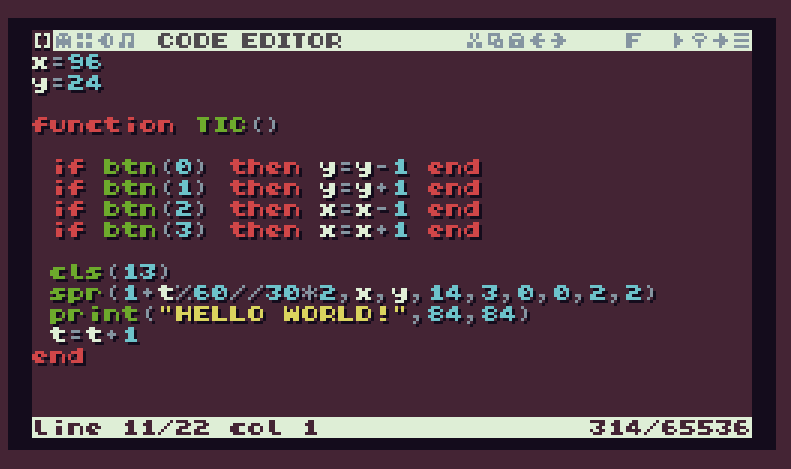
\includegraphics[width=1\linewidth]{enviro.png}

\section{Getting started}
\begin{enumerate}
	\item Go onto the TIC-80 website by searching for TIC-80 on a search engine.
	\item Click on the \textbf{CREATE} tab on the navigation bar. Then click on the \textbf{CLICK TO START...} box to start open the program. If you want to save your work or if the internet is slow for you, you can download an offline version of the program.
	\item You will now be greeted by the ``Command Line'' of TIC-80. We will be doing a \textit{very} quick rundown of the command line.
	\begin{enumerate}
		\item Press escape on your keyboard to toggle between the Editor and Command Line.
		\item When you get to the editor, you will see some default code. For now we will leave it alone. Just scroll down a little bit so you can see it all.
		\item Press escape again to toggle back to the command line. If you type \lstinline{run}, the command line will run all of the code that is currently in your editor. You should see this picture.
		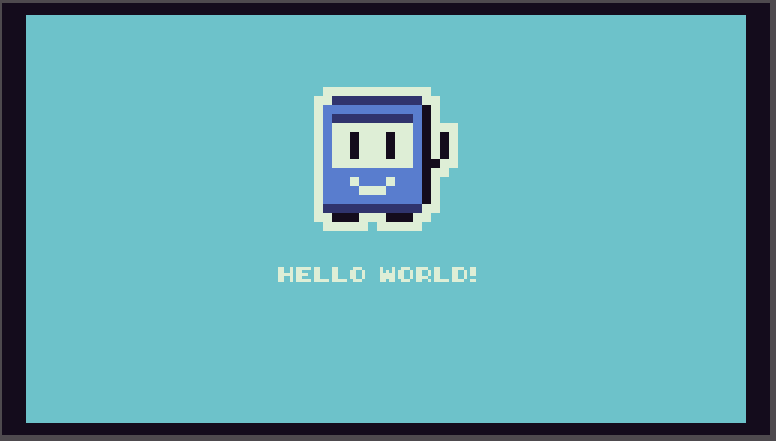
\includegraphics[width=1\linewidth]{default_game.png}
		\item Press escape again to exit the game back to the command line.
		\item That's it! :)
	\end{enumerate}
	\item Now that you have an idea of how to run a game, it's time to create one. Open up the editor.
\end{enumerate}

\section{Creating your first TIC-80 game}
In this section we will be going over the very basics of creating a game with TIC-80. We will be creating pong since pong is basically the ``Hello world'' of video game creation.
\begin{enumerate}
	\item Delete the code until it looks like the picture below. Also edit the top \textbf{three} lines to suit your game. Don't edit \lstinline{--script}. 
	
	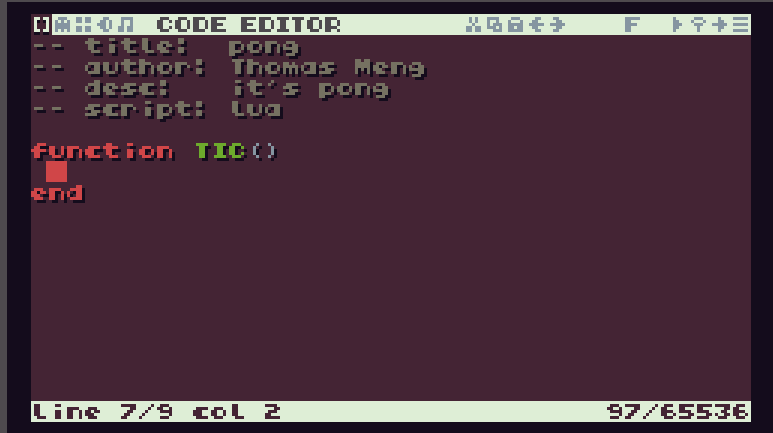
\includegraphics[width=1\linewidth]{game_base.png}
	
	The \lstinline{function TIC()} is basically the equivalent to a forever loop in Scratch. In TIC-80, there is only a single loop rather than as many loops as you want in Scratch. The basic difference is that you will have to check for button presses and tell things to move around in the same loop.
	
	The loop is ended by the \lstinline{end} keyword; everything in between will be repeated for as long as the game is running. If you run your game now, you will notice that nothing will be drawn to the screen.
	\item We will begin the script by drawing our pong paddle.
\end{enumerate}

\end{document}
